%______________________________________________________________________________
% main.tex

\input{preamble12-screen.tex}
\hypersetup{%
    pdfauthor={Mike Pierce}%
   ,pdftitle={Math N16B Homework Six, Summer 2021}%
   ,pdfkeywords={Pierce,MathN16B,16B,N16B,Calculus,Integration,Berkeley}%
}
\usepackage{fourier}
\input{accessible-colors.tex}
\input{newcommand.tex}
\input{newenvironment.tex}
\pagestyle{empty}


\begin{document}

\begin{center}
    {\Huge{Homework Six}}
    \\ \footnotesize{Analytic Geometry and Calculus}
    \\ \footnotesize{UC Berkeley Math N16B, Summer 2021}
\end{center}
\vspace{2em}

Upload your responses to the prompts marked
(\textsc{\textcolor{magenta}{Submit}})
to Gradescope before 8pm Friday; 
you will receive feedback on these.
\begin{center}
    \href{https://www.gradescope.com/courses/275664}%
    {\texttt{gradescope.com/courses/275664}}
\end{center}
The rest of the exercises you should complete at your discretion.
Note that \emph{Calculus with Applications, 11th Edition} 
has some select solutions, usually to odd-numbered exercises, in the back.


\section*{Goals this Week}

Here are some goals you should have in mind while exercising:
\begin{enumerate}
    \item 
        Learn to solve a linear first-order ODE. 
        It's just a procedure/calculation to practice a few times.
        You'll get some practice at this while studying applications of ODEs too.
    \item 
        Understand Euler's method of approximating the solution to an ODE,
        and relate this understanding to an ODE's direction (vector) field.
        This is also related to a broad theme of calculus:
        linear approximations are easy to compute
        and often good enough for whatever you're doing.
    \item 
        The study of differential equations is born from the 
        art of applying mathematics to study the natural world. 
        This introduction to ODEs was brief, but you should
        familiarize yourself with as many applications of ODEs
        as you can before we go.
\end{enumerate}

\newpage

\section*{Exercises}

\begin{enumerate}
    \item % 10.2 Linear ODEs and Integrating Factors
        I expect you to be able to recognize a linear first-order
        differential equation when you see one and then solve it if you want.
        The initial exercises from Chapter 10.2 of 
        \emph{Calculus with Applications, 11th Edition}
        provides you with plenty of drills to practice.

    \item 
        Give me an example of a single variable function
        such that the derivative of the function is equal to 
        one more than the function.

    \item
        With this exercise you'll practice some symbol-pushing.
        \begin{center}
            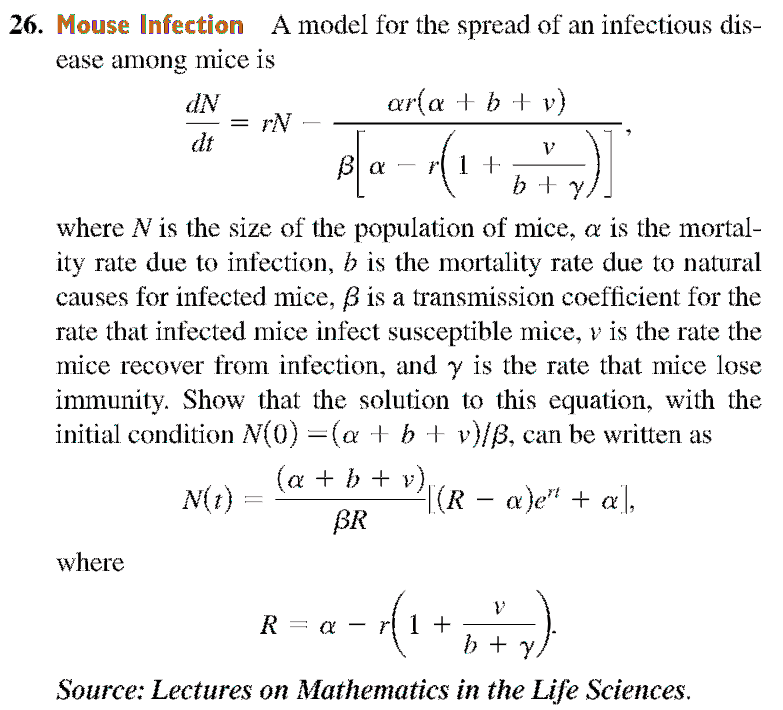
\includegraphics[width=0.96\textwidth]{screenshots/26.png}
        \end{center}

    \item % 10.3 Euler's Method and Numerical Approximation
        I expect you to \emph{understand} Euler's method of approximating
        a solution to an ODE, but the actual calculations are tedious
        and should never be done by hand; morally this is something you
        should only be programming a computer to do.
        So only do the initial exercises from Chapter 10.3 of 
        \emph{Calculus with Applications, 11th Edition}
        if you really feel you need to. 
        Otherwise I think it'd be more fruitful to you 
        to just read about Euler's method and listen to folks explain it
        until you get the idea.

    \item % 10.4 Applications
        You might want to read over the way 
        \emph{Calculus with Applications, 11th Edition}
        models continuous financial deposits in Chapter 10.4 
        before looking at these exercises.
        \begin{center}
            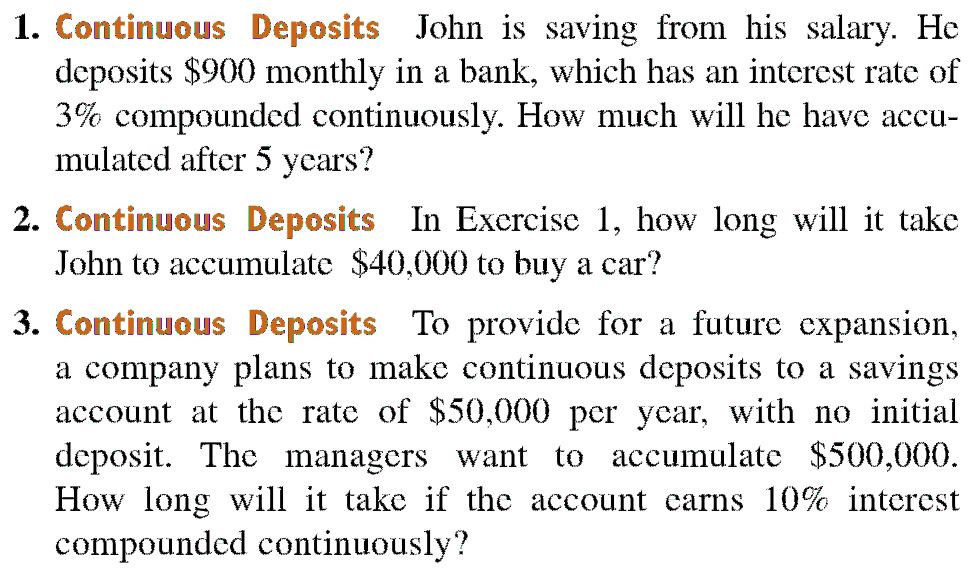
\includegraphics[width=0.96\textwidth]{screenshots/123.png}
        \end{center}

    \newpage

    \item 
        A flock of turkeys in a region will grow at a rate 
        that is proportional to its current population. 
        In the absence of any outside factors 
        the population will triple in $5$ days. 
        On any given day about $3$ turkeys die of natural causes,
        $9$ turkeys are taken by hunters, and $2$ turkeys 
        wander into the flock from neighboring regions.
        If there are initially $50$ turkeys in the flock 
        will the flock survive or die out? 

    \item % 10.4 Applications
        You might want to read over the way the textbook 
        (\emph{Calculus with Applications, 11th Edition}) 
        models a predator/prey situation
        in Chapter 10.4 before looking at these exercises.
        \begin{center}
            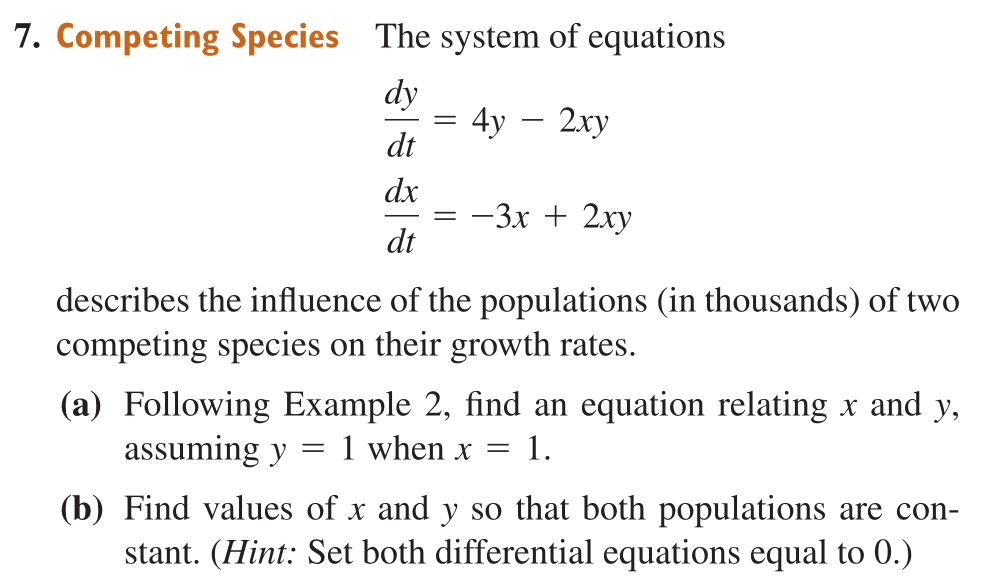
\includegraphics[width=0.96\textwidth]{screenshots/7.png}
        \end{center}
        \newpage
        %(\textsc{\textcolor{magenta}{Submit}}) this one
        \begin{center}
            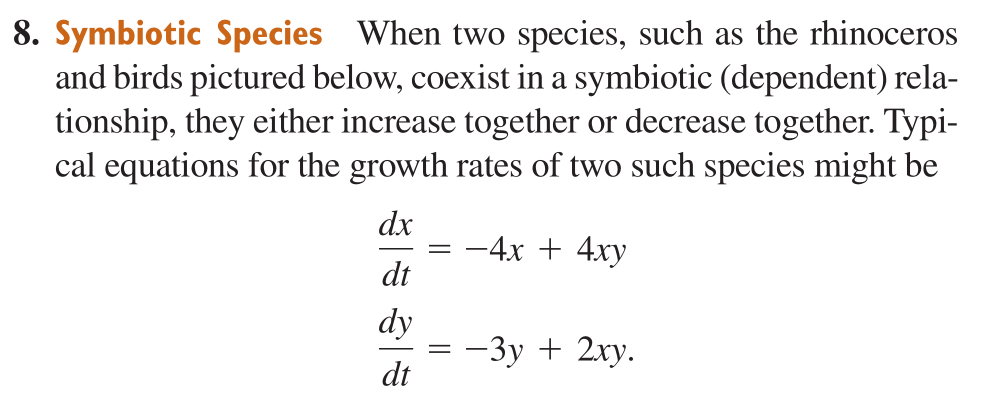
\includegraphics[width=0.96\textwidth]{screenshots/8-1.png}
            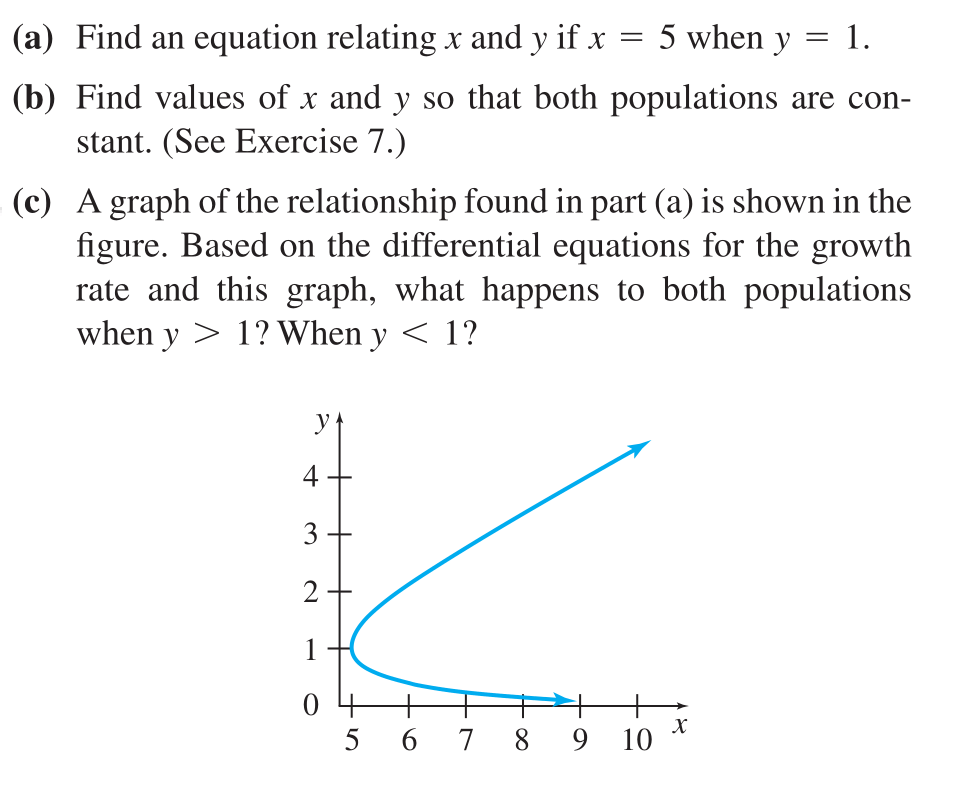
\includegraphics[width=0.96\textwidth]{screenshots/8-2.png}
        \end{center}

    \newpage

    \item % 10.4 Applications
        A few more exercises from the textbook.
        \begin{center}
            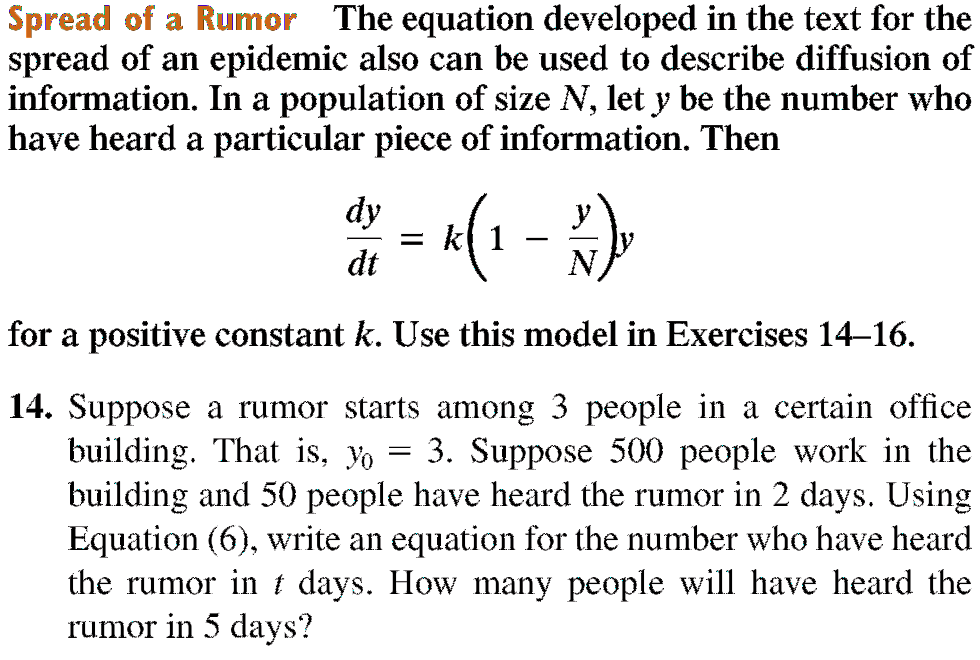
\includegraphics[width=0.96\textwidth]{screenshots/rumor-1.png}
            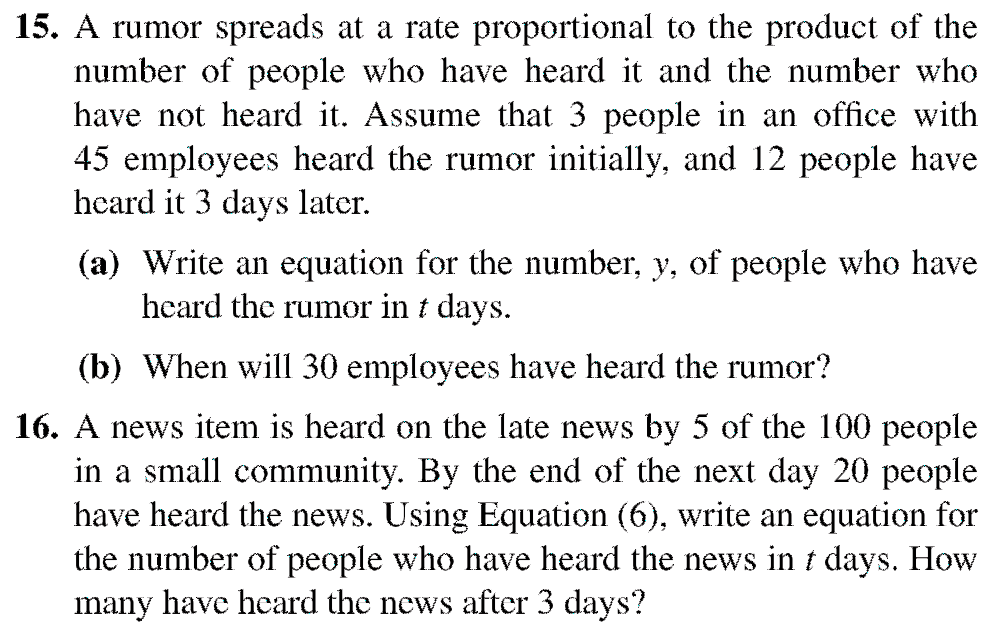
\includegraphics[width=0.96\textwidth]{screenshots/rumor-2.png}
        \end{center}

    \newpage

    \item % 10.4 Applications
        Yet a few more exercises from the textbook.
        \begin{center}
            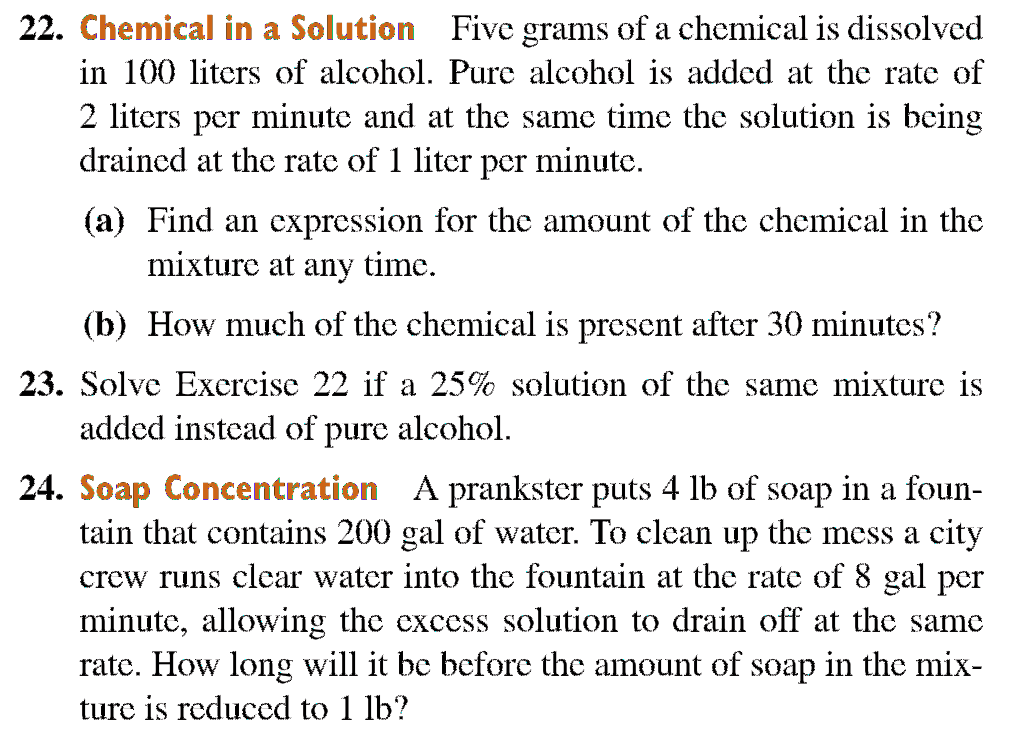
\includegraphics[width=0.96\textwidth]{screenshots/222324.png}
        \end{center}

    \item 
        (\textsc{\textcolor{magenta}{Submit}})
        Consider a tank used in certain hydrodynamic experiments.
        After one experiment the tank contains $200$ liters of a dye solution 
        with a concentration of $1\,\mathrm{g/liter}$. 
        To prepare for the next experiment, 
        the tank is to be rinsed with fresh water flowing in 
        at a rate of $2 \,\mathrm{liters/min}$, 
        and the well-stirred solution will flow out at the same rate.
        How much time will have to elapse before the amount 
        of the dye in the tank reaches $1\%$ of its original value?

\end{enumerate}
\newpage

The following model is not covered in the textbook, 
which is strange.
It is a rather fundamental differential equation that models 
the acceleration/velocity of a falling object. 
In particular, if an object is falling towards a planet
with gravitational constant $g$, then the velocity of that object 
is described by the equation $\dot{v} = g - kv$, where $k$ is some constant.
The idea is that the amount of air resistance 
that an object experiences while falling is proportional to its velocity;
that's the whole idea behind the $-kv$ term.
And obviously there's an independent variable $t$ for time 
underlying this model, 
even though it's not explicitly required to describe $\dot{v}$.

\begin{enumerate}[resume]

    \item
        Suppose you throw a $3\,\mathrm{kg}$ 
        watermelon off the top of a tall building downward 
        towards the parking lot below
        with an initial velocity of $17\,\mathrm{m/s}$.
        While falling, the force of air resistance on your watermelon
        is $3$ times the velocity of the falling melon.
        Write down a function that returns the velocity $v(t)$
        of the watermelon after $t$ seconds of being thrown. 
        How long after being thrown will the watermelon 
        be traveling at $11\,\mathrm{m/s}$?

        \textsc{Hint}: Recall that acceleration due to gravity near
        the surface of the earth is given by $9.81\,\mathrm{m/s^2}$,
        but I think for the sake of making calculations easier
        you should just round that number to $10\,\mathrm{m/s^2}$.

    \item
        (\textsc{\textcolor{magenta}{Submit}})
        A stone having a mass of $2\,\mathrm{lbs}$  
        is dropped from a bridge with no initial velocity,
        and encounters air resistance that is exactly equal 
        to the square of its velocity.
        What is the velocity of the stone after $1$ minute?
        For this question use imperial units, so acceleration
        due to gravity is $32\,\mathrm{ft/s^2}$ 
        instead of the usual metric $9.81\,\mathrm{m/s^2}$.

    \item
        A ball of mass $3$ grams is thrown vertically into the air
        with an initial velocity $12 \,\mathrm{m/s}$. 
        Suppose the ball encounters an air resistance 
        equal to $5$ times its velocity.
        Find a function $v(t)$ that returns the velocity of ball
        at a given time $t$. How long after being thrown upward
        does the ball reach its maximum height?

    \item \label{item:smart}
        Suppose that there is a plane flying over the earth,
        equipped with a cannon that is pointed towards the earth.
        The cannon shoots a $2\,\mathrm{kg}$ cannonball at earth 
        at an initial speed of $300\,\mathrm{ft/s}$. 
        But this is no ordinary cannonball;
        this is a Smart Cannonball\texttrademark{}.
        After being fired it will gradually reconfigure its shape 
        to become more aerodynamic to reduce air resistance.
        Following the convention that forces acting on the 
        cannonball in the direction away from earth are negative,
        the Smart Corporation estimates that after $t$ seconds of being fired
        the force from air resistance exerted on the cannonball 
        will be$-\frac{v}{1+t}$, where $v$ is the velocity of the cannonball
        at time $t$.

        Using this new estimate for the force of air resistance
        on the cannonball, write down a differential equation
        that models the motion of the cannonball. 
        Then find a function $v(t)$ that returns the velocity 
        of the cannonball after $t$ seconds of being fired.

        Calculate the limit $\lim\limits_{t \to \infty} v(t)$.
        Does the differential equation you developed 
        have any equilibrium solutions?
        Based on this information, what can you conclude
        about the accuracy of Smart Corporation's claim
        that the force from air resistance will be given by
        $-\frac{v}{1+t}$ after $t$ seconds?

    \item 
        (\textsc{Recreation})
        Five women and a monkey were shipwrecked on a desert island.
        They spent the first day gathering coconuts for food,
        piling up all the coconuts together 
        before they went to sleep for the night. 
        But while they were all asleep, one woman woke up and thought 
        there might be a row about dividing the coconuts in the morning, 
        so she decided to get up and take her share now. 
        She divided the coconuts into five equal piles except for
        one coconut left over which she gave to the monkey, 
        and she hid her pile and put the rest back together. 
        By and by, another woman woke up and did the same thing,
        and similarly she had one coconut left over 
        which she gave to the monkey. 
        And each of the five women did the same thing, one after the other; 
        each one taking a fifth of the coconuts in the pile when she woke up, 
        and each one having one left over for the monkey. 
        In the morning they divided what coconuts were left, 
        and they came out in five equal shares. 
        Of course each one must have known that there were coconuts missing,
        but each one was as guilty as the others, 
        so they didn't say anything. 
        How many coconuts were there in the beginning?

\end{enumerate}

\end{document}
